\documentclass[11pt, oneside]{article}   	% use "amsart" instead of "article" for AMSLaTeX format
\usepackage{geometry}                		% See geometry.pdf to learn the layout options. There are lots.
\geometry{letterpaper}                   		% ... or a4paper or a5paper or ... 
%\geometry{landscape}                		% Activate for for rotated page geometry
%\usepackage[parfill]{parskip}    		% Activate to begin paragraphs with an empty line rather than an indent
\usepackage{graphicx}				% Use pdf, png, jpg, or eps§ with pdflatex; use eps in DVI mode
								% TeX will automatically convert eps --> pdf in pdflatex		
\usepackage{amssymb}
\usepackage{amsmath}

\title{Homework 8 - CS 6210}
\author{Ally Warner}
%\date{}							% Activate to display a given date or no date

\begin{document}
\maketitle

\section{Grid}

Create triangular finite element grids of different resolution by dividing the finite difference grids squares you created in Homework 7 into two triangles.

To crease my triangular finite element grid, I calculated the size of the grid based on the input of $h$, which is the distance between nodes on our grid. I used my method from homework 7 to find the physical positions of the nodes in relation to the grid. I then made a mesh by saving the nodes that made up each element in a matrix. I used triplot to visualize my grid. The following figures show my triangular mesh with different values of $h$. \\

\centerline{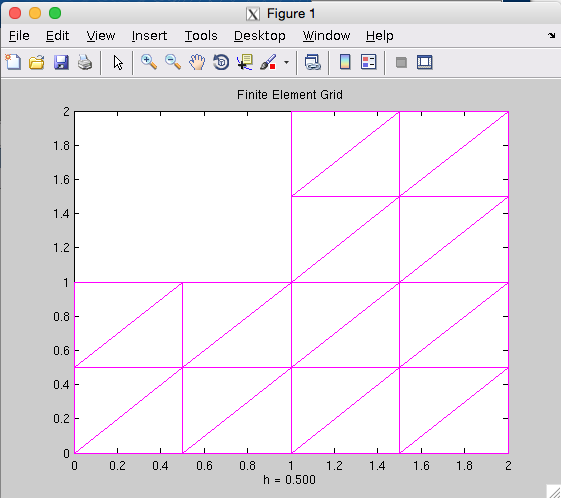
\includegraphics[scale = 0.55]{Grid_h1.png}}

\vspace{5mm}

\centerline{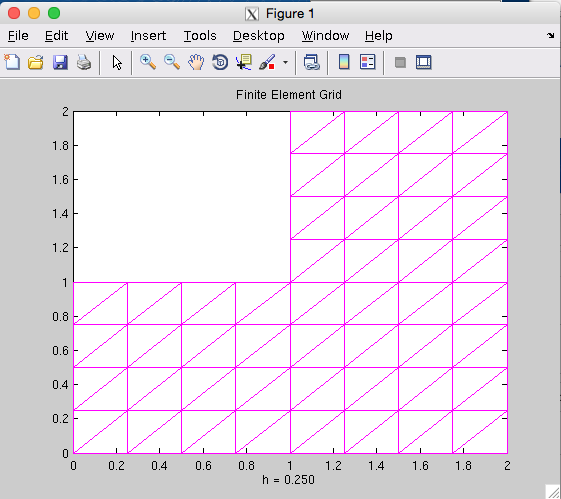
\includegraphics[scale = 0.55]{Grid_h2.png}}

\vspace{5mm}

\centerline{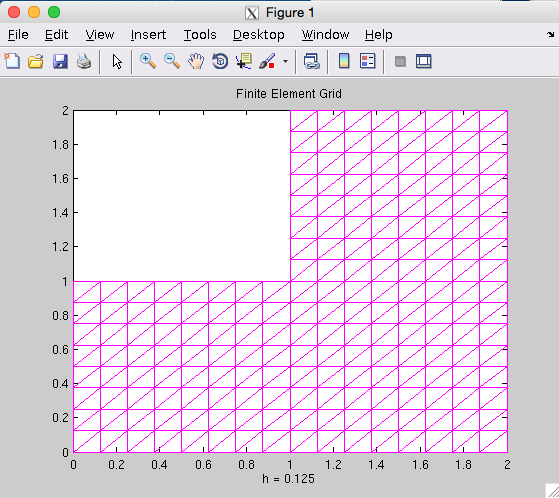
\includegraphics[scale = 0.55]{Grid_h3.png}}

\vspace{5mm}

\centerline{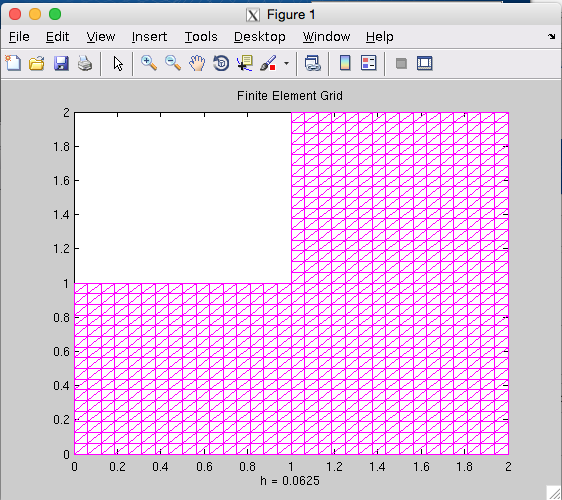
\includegraphics[scale = 0.55]{Grid_h4.png}}

\vspace{5mm}

\centerline{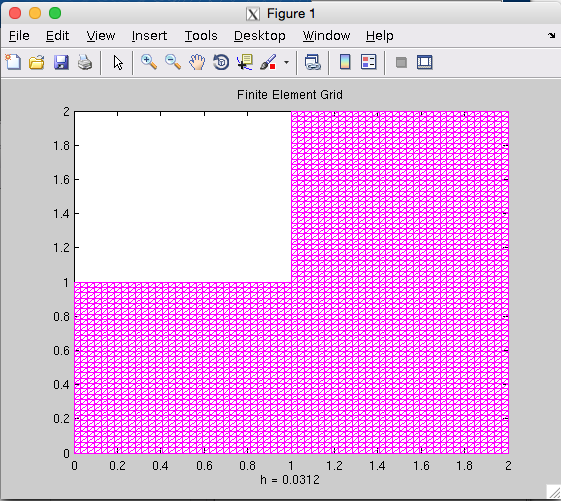
\includegraphics[scale = 0.55]{Grid_h5.png}}

\vspace{5mm}

\section{Finite Element Method}

Writing a finite element method was a bit more complex than writing the finite difference method code. First, we take our positions of nodes and the mesh information and we find the physical position of the vertices of each element. From this we can make our local matrices which need first order triangular elements. After we have made these, I save their row information into three separate matrices. I then make the global matrix by looping throw these row matrices. After the global matrix has been made, the boundary conditions are applied and there is a linear system to solve! The solved linear system is shown in the following figures at different values of $h$. \\

\centerline{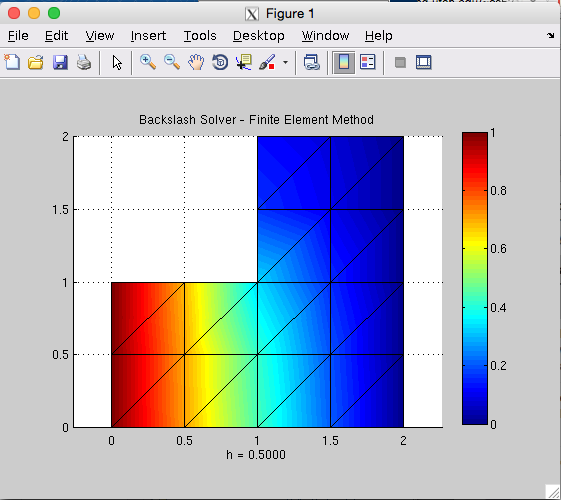
\includegraphics[scale = 0.55]{Backslash_h1.png}}

\vspace{5mm}

\centerline{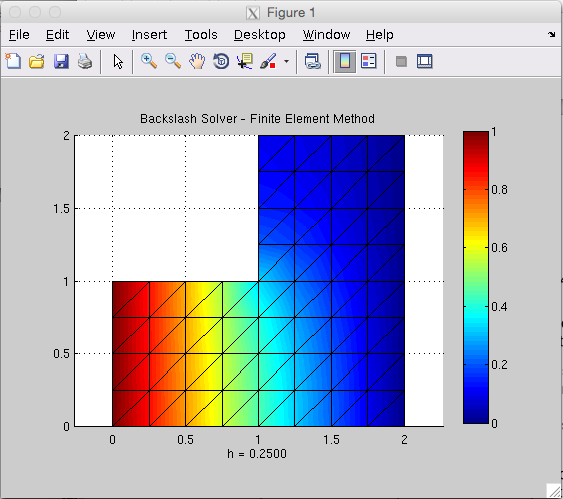
\includegraphics[scale = 0.55]{Backslash_h2.png}}

\vspace{5mm}

\centerline{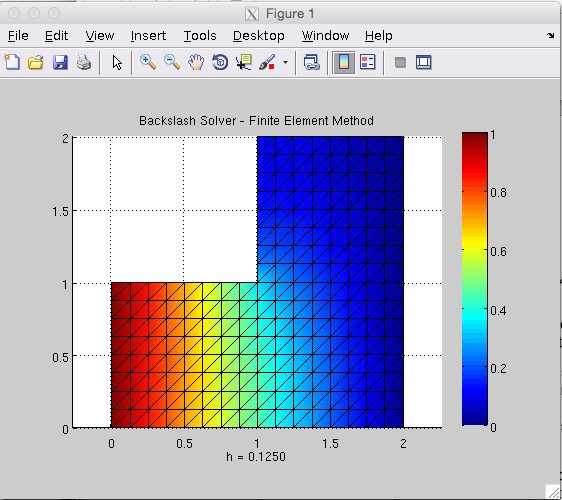
\includegraphics[scale = 0.55]{Backslash_h3.png}}

\vspace{5mm}

\centerline{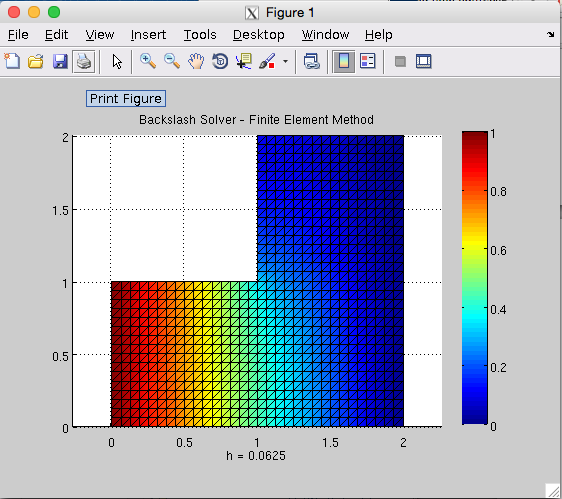
\includegraphics[scale = 0.55]{Backslash_h4.png}}

\vspace{5mm}

\centerline{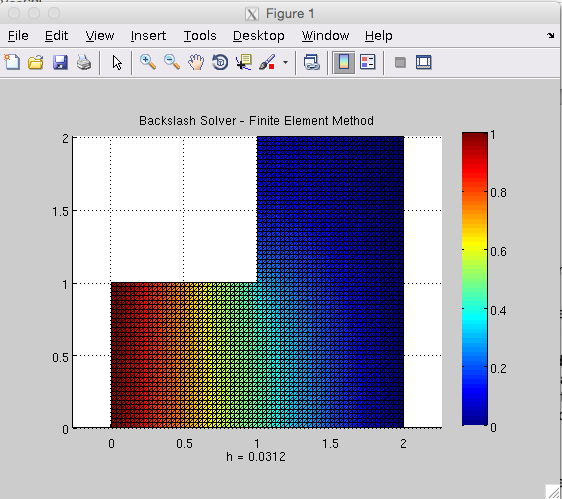
\includegraphics[scale = 0.55]{Backslash_h5.png}}

\vspace{5mm}

\section{FEM and FDM Comparison}

I solved the steady state heat problem using the finite element method and the finite difference method and compared their run time, using the backslash solver, and their solutions via contour plots. The cpu time comparison is shown in the table below. \\

\centerline{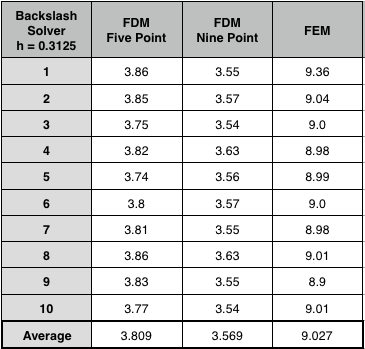
\includegraphics[scale = 0.7]{TimeComparisons.png}}

\vspace{5mm}

As you can see, the finite element method is about three times slower than finite difference method. Although this method is slower, it is more accurate. This can be seen from the contour plots in the following figures. \\

\centerline{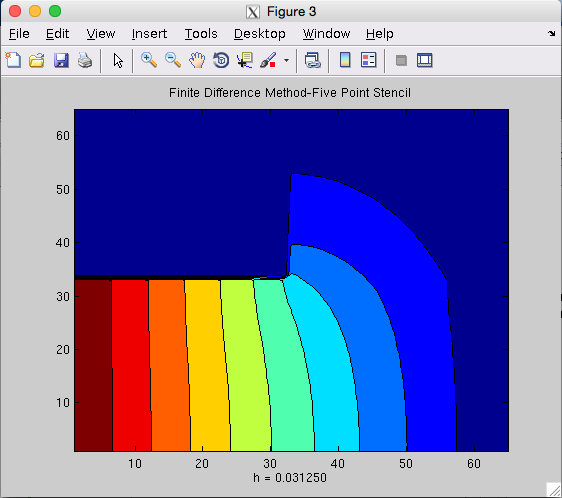
\includegraphics[scale = 0.55]{FDM_fivePoint.png}}

\vspace{5mm}

\centerline{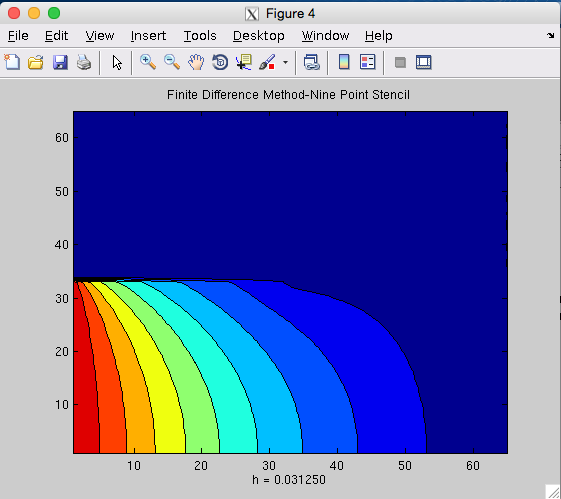
\includegraphics[scale = 0.55]{FDM_ninePoint.png}}

\vspace{5mm}

\centerline{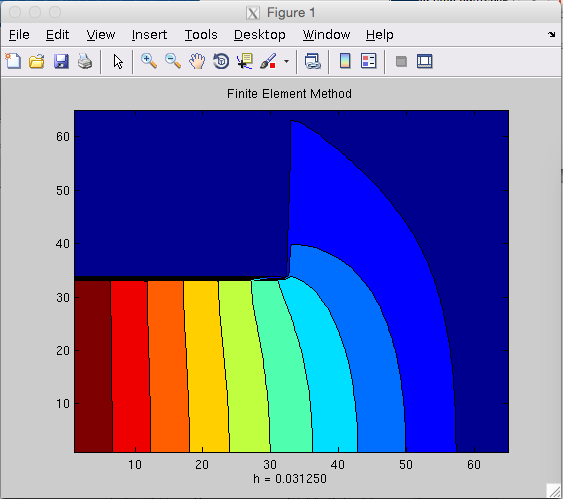
\includegraphics[scale = 0.55]{FEM_contour.png}}

\vspace{5mm}

\section{Delaunay}

Last, we get to work with an unstructured grid. After loading in the delaunay file and removing the extra points, I ran it through my original code and had a grid and a solution shown in the following figures. \\

\centerline{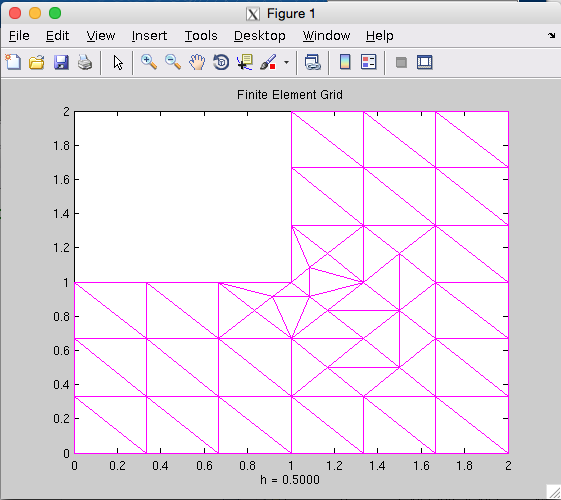
\includegraphics[scale = 0.55]{UnstructuredGrid.png}}

\vspace{5mm}

\centerline{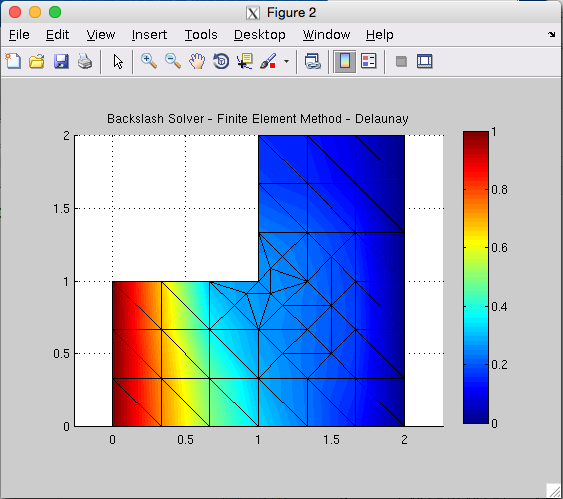
\includegraphics[scale = 0.55]{FEM_unstructured_1.png}}

\vspace{5mm}

In comparison to our structured grid, we know that this is quite the right answer. So adding nodes to the grid can help the solution to become more accurate. Figure out how adding nodes in specific places of the grid affects the solution was a bit tricky at first. The figure shown below shows my first pass at making the solution more accurate. \\

\centerline{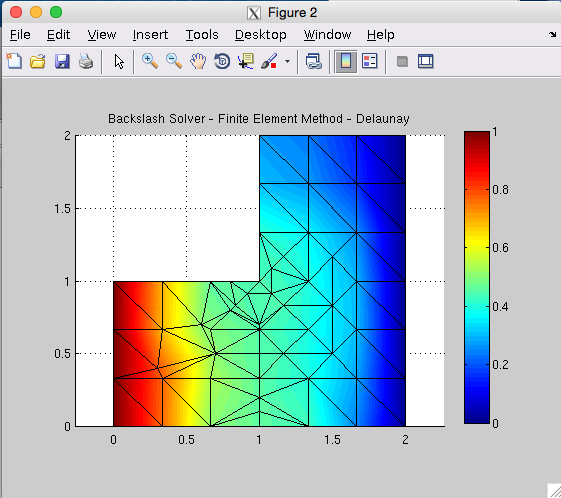
\includegraphics[scale = 0.55]{FEM_unstructured_2.png}}

\vspace{5mm}

We can see that this isn't a very accurate solution at all. So instead of adding many points at once, I just added one point at a time to see how to "push" the solution to be more accurate. My second attempt at making the solution is much better and shown below with the corresponding grid. \\

\centerline{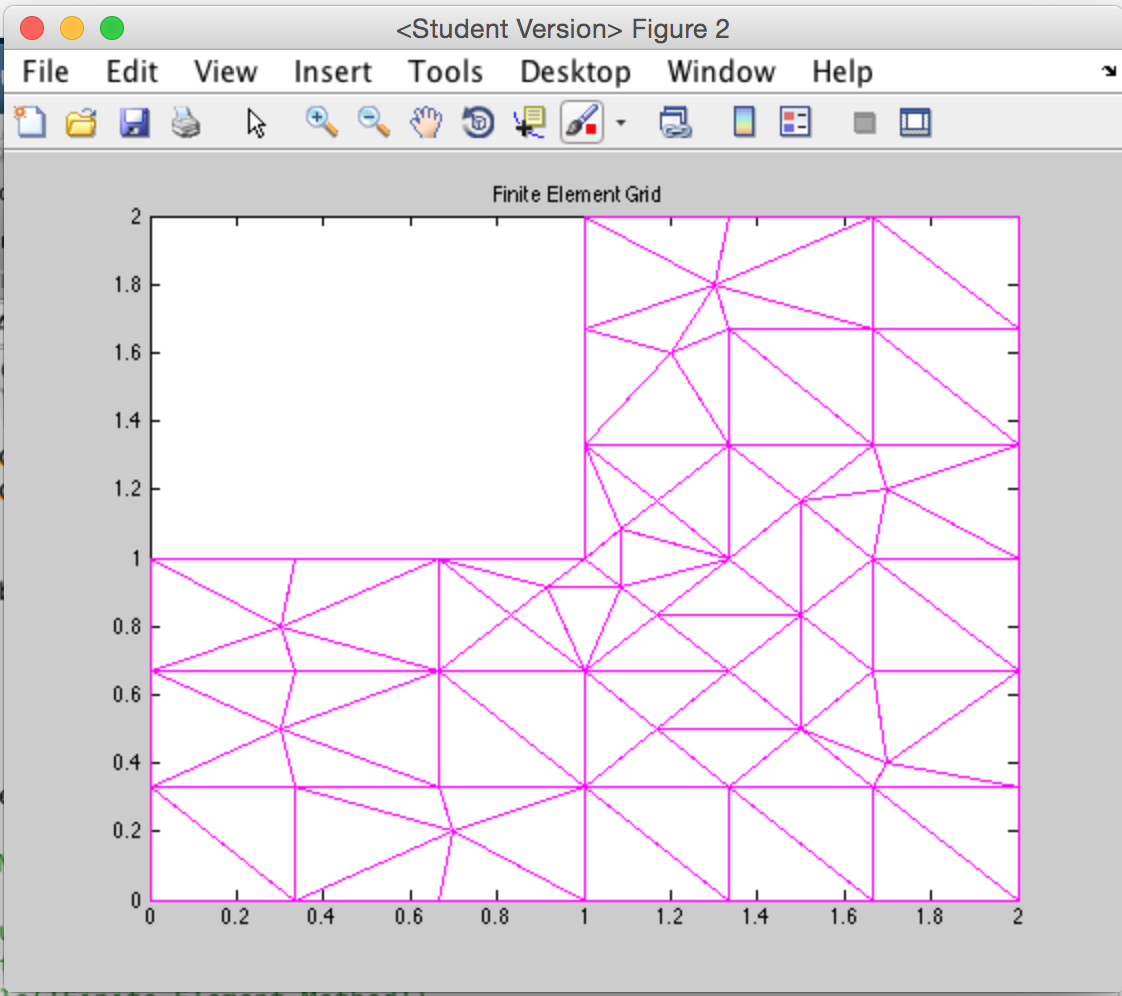
\includegraphics[scale = 0.55]{DelaunayAdjustGrid.png}}

\vspace{5mm}

\centerline{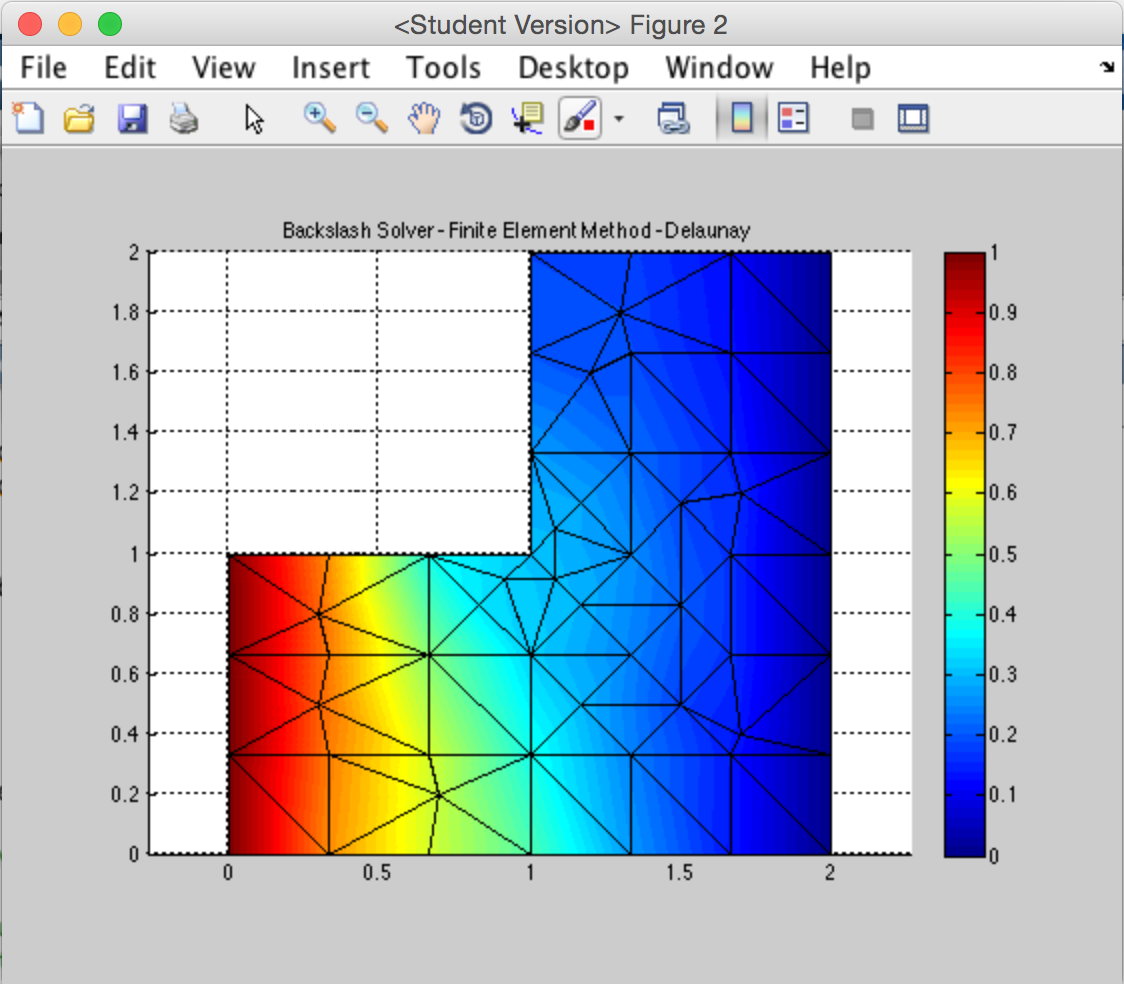
\includegraphics[scale = 0.55]{DelaunayAdjust.png}}

\vspace{5mm}

*All of the code for this assignment is submitted with the assignment.

\end{document}  